\chapter{Data Storage - Computer Science Papers Dataset}

\section{The Data Model}
\paragraph{ }The data used for this task was taken from the \texttt{dblp} computer science bibliography dataset\footnote{https://dblp.uni-trier.de/xml/}. This data came in the form of an XML file. The interesting features from this file were extracted and stored as a graph database (using Neo4J) in order to perform the required analysis. The chosen model was quite a simple one and can be seen in Figure \ref{fig::model} where there are two types of nodes (\texttt{Article} and \texttt{Author}) and 1 relationship (\texttt{PUBLISHED}).

\begin{figure}[!b]
	\centering
	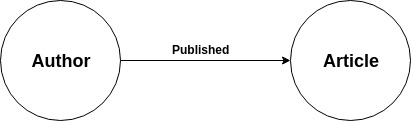
\includegraphics[width=0.6\textwidth]{model}
	\caption[Neo4J Model]{Graph Model Used to Store the \texttt{dblp} Data in Neo4J}
	\label{fig::model}
\end{figure}

\paragraph{ }The \texttt{Author} node simply contains the name of the author. This field was also set as the key since according to the documentation of \texttt{dblp} the name is stored in a way which is guaranteed to be unique. The \texttt{Article} Node, despite its misleading name, stores data on any of the publications listed in the \texttt{bdlp} dataset. This includes articles,articles in proceedings, proceedings, books, articles in collections, PhD thesis, Masters thesis and publications from web sources. These nodes have 2 fields; a key field which contains the unique key identifier assigned to them in the \texttt{dblp} database and the title field containing the name of the publication. Finally, the relationship \texttt{PUBLISHED} contains no fields as it wasn't necessary.

\paragraph{ }In order to import the data into Neo4J, the following steps were done:
\begin{itemize}
	\item Firstly, Neo4J was installed on the local machine. The command \texttt{sudo service neo4j status} was used to check the status of the server and since it was inactive \texttt{sudo service neo4j start} was used to start the server.
	\item The Jupyter Notebook code in `01 - Data Extraction.ipynb' was run to create the data files.
	\item The generated data files were then copied to the Neo4J import directory by running \texttt{sudo cp [file.csv] /var/lib/neo4j/import/[file.csv]} .
	\item Finally, some quotes found in titles of the publications were removed by running \texttt{sudo sed -i 's/\"//g' articles.csv}
\end{itemize}
In particular, in the python file, \texttt{lxml} was first used to extract the required features from the xml file into three csv files (one for each node and one for the relationship). This was slightly tricky to handle due to the size of the xml file and the amount of memory available on the laptop used to run this program. Thus, a generator function was used that would access the xml file element by element rather than storing the whole file in memory. Similarly, the csv files were accessed only when needed in order to ensure that not too much memory we being used. This was a necessary step that traded speed for memory. \texttt{py2neo} was then used to access the database, set the uniqueness constraints on the desired fields in the nodes and load the csv data.

\section{Some Cypher Queries}
\paragraph{ }After loading everything on Neo4J, some queries were run in Cypher using \texttt{py2neo} to explore the dataset. In particular; the amount of \texttt{Article} nodes were counted and it was found that there are a total of 6,661,235 nodes, the amount of actual articles were counted and it was found that there are a total of 1,956,852, and the author that published the most articles was found to be H. Vincent Poor, who published 1,568 articles! The following queries were used to obtain this information:\\

Count the number of \texttt{Article} nodes:
\begin{verbatim}
MATCH (n:Article) RETURN count(*)
\end{verbatim}
Count the number of articles:
\begin{verbatim}
MATCH (n:Article) WHERE n.key STARTS WITH `journals' 
RETURN  count(*)
\end{verbatim}
Get the top 10 authors that published the most amount of articles:
\begin{verbatim}
MATCH (a:Author)-[p:PUBLISHED]-(:Article)
RETURN a.name, count(p) as rel_count
ORDER BY rel_count desc LIMIT 10
\end{verbatim}

\section{Authorship Sub-Graph}

\begin{figure}[!b]
	\centering
	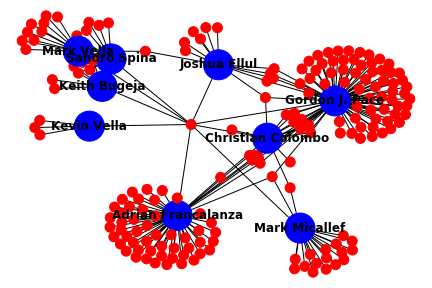
\includegraphics[width=0.6\textwidth]{cs_department}
	\caption[Department Sub-Graph]{Authorship Sub-Graph of the CS Department at UoM}
	\label{fig::cs_department}
\end{figure}

\paragraph{ }Figure \ref{fig::cs_department} was then extracted to show the authorship subgraph for members of the Computer Science department at the University of Malta. The list of members was taken from the department website\footnote{https://www.um.edu.mt/ict/cs/about/staff}. The following Cypher query was then used to extract the nodes as required:
\begin{verbatim}
MATCH (a:Author)-[p:PUBLISHED]->(b:Article)
WHERE a.name in [`Kevin Vella',`Keith Bugeja',`Christian Colombo',
    `Joshua Ellul',`Adrian Francalanza',`Mark Micallef',
    `Gordon J. Pace',`Sandro Spina',`Mark Vella',
    `Kevin Cortis']
RETURN a,p,b
\end{verbatim}
The extracted table was then converted into a \texttt{pandas} data-frame and \texttt{networkx} was used to display the extracted sub-graph.

\section{Shortest Paths}

\begin{figure}[!b]
	\centering
	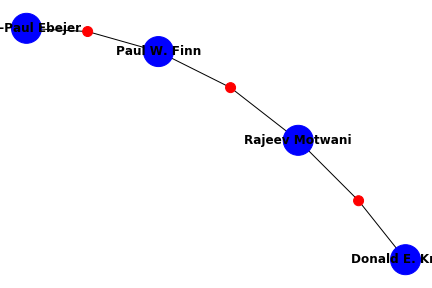
\includegraphics[width=0.6\textwidth]{knuth}
	\caption[Shortest Path]{Path from Jean-Paul Ebejer to Donald E. Knuth}
	\label{fig::knuth}
\end{figure}


\paragraph{ }The shortest path function in Cypher was then used to find the shortest path between two different authors. The first query was run to show one of the shortest paths that exist from Dr Jean-Paul Ebejer to Prof. Gordon Pace from the University of Malta in order to test out the function between two authors that are known to be closely connected.
\begin{verbatim}
MATCH (p1:Author {name:'Jean-Paul Ebejer'}),
    (p2:Author {name:'Gordon J. Pace'}),
    path = shortestpath((p1)-[:PUBLISHED*]-(p2))
RETURN path
\end{verbatim}
The second query was then run to find the shortest path between Jean-Paul Ebejer and Donald E. Knuth.
\begin{verbatim}
MATCH (p1:Author {name:'Jean-Paul Ebejer'}),
    (p2:Author {name:'Donald E. Knuth'}),
    path = shortestpath((p1)-[:PUBLISHED*]-(p2))
RETURN path
\end{verbatim}
It was found that a connection actually does exist between these two authors and the path returned can be seen in figure \ref{fig::knuth}.

\section{Erd\H{o}s Numbers}

\begin{figure}[!b]
	\centering
	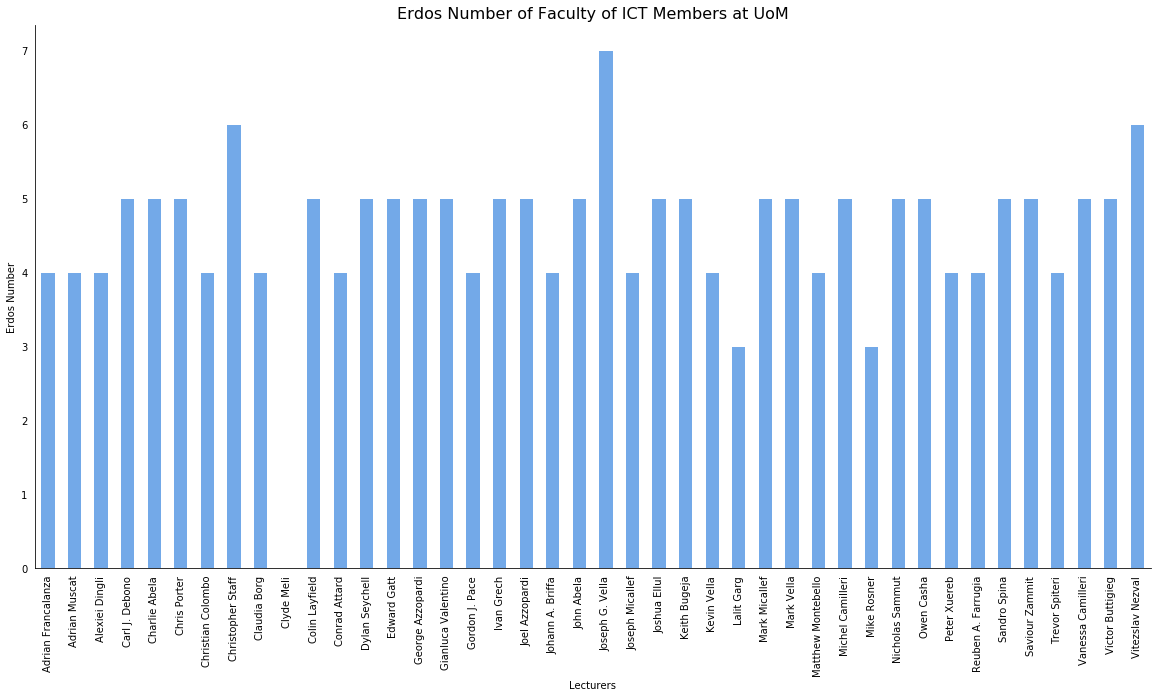
\includegraphics[width=\textwidth]{erdos}
	\caption[Erd\H{o}s Numbers]{Erd\H{o}s Numbers for members of the Faculty of ICT at UoM}
	\label{fig::erdos}
\end{figure}

\paragraph{ }A function was then written to extract the Erd\H{o}s Number of a given author. The function made use of the following query (where \texttt{NAME} refers to the author name passed to the function):
\begin{verbatim}
MATCH (p1:Author {name: NAME}),
    (p2:Author {name:'Paul Erd&#246;s'}),
    path = shortestpath((p1)-[:PUBLISHED*]-(p2))
RETURN length(path)
\end{verbatim} 
The Erd\H{o}s Number of Dr. Jean-Paul Ebejer was then found to be 4. Finally, figure \ref{fig::erdos} was plotted to show the Erd\H{o}s Numbers of the members of the Faculty of ICT at UoM. Note that the members of the faculty were taken from each department's website. A histogram was also plotted for the Erd\H{o}s numbers to further show the distribution of these values and can be seen in figure \ref{fig::hist_erdos}.

\begin{figure}[!t]
	\centering
	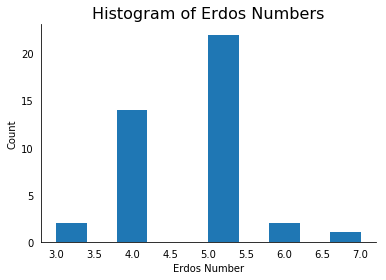
\includegraphics[width=0.6\textwidth]{erdos_hist}
	\caption[Erd\H{o}s Numbers Histogram]{ Histogram of Erd\H{o}s Numbers for members of the Faculty of ICT at UoM}
	\label{fig::hist_erdos}
\end{figure}

\section{Six Degrees of Separation}
